
% 本教程2019-7-20 前由 Yushu Xu 维护
% 2019-7-20 起由 Tongxin Ren  维护



\documentclass[12pt]{elegantpaper} % 源文件的类型
%============================================================
%                     宏包区
%============================================================
\usepackage{graphicx}
\usepackage{subfig}

\usepackage{multirow}
\usepackage{booktabs}  % 制作三线表
\usepackage{diagbox}   % 表格中的斜线
\usepackage{makecell}  % 垂直合并单元格

%============================================================
%                     标题区
%============================================================
\title{\LaTeX : 插图与插表}
% 作者
\author{任公子@SJTU}
% 日期
\date{\today}  
\begin{document}
\maketitle   %生成标题页
\newpage
%============================================================
\section{插图}




\subsection{基本插图方法}


允许的图片格式:pdf / jpg / png / eps / bmp

基本环境定义格式:
% \includegraphics 的可选参数: width,height,scale
% \textwidth 文本行的宽度
% \linewidth 行的宽度,一般来说等于textwidth
% 0.5\linewidth  这里的0.5是指一行放两个图,如果放三个是0.33\linewidth
\renewcommand{\figurename}{图 }

\begin{figure}[htbp]	
	\centering	
	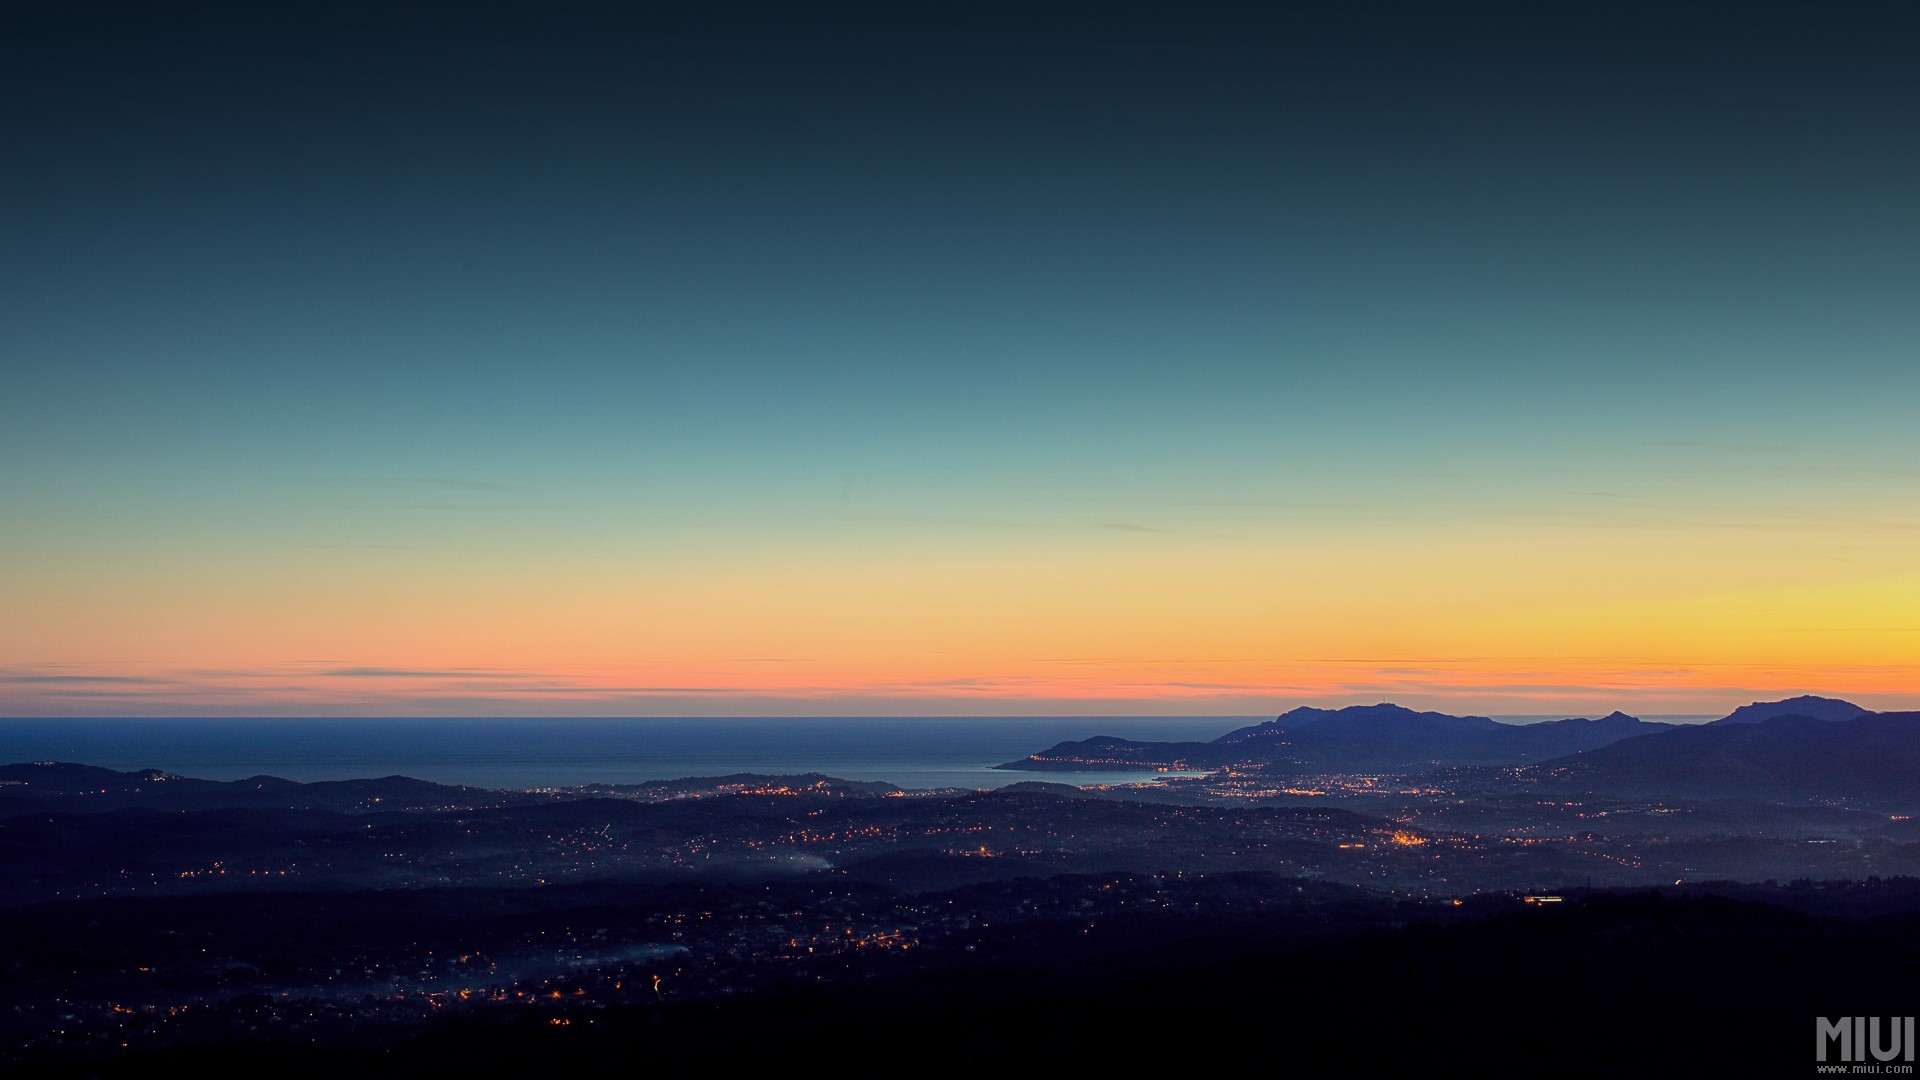
\includegraphics[width=0.5\textwidth]{figure/demo.jpg}	
	\caption{我的图片标题}	
    \label{demo1}      % label一定要在caption之后定义
\end{figure}


% 图片的引用
according to the picture Figure(\ref{demo1}), .......


\subsection{并列插图方法}


水平插入两张图片
% minipage 的可选参数:l:左对齐 c:居中 r:右对齐
% 必选参数:图片占的宽度
\begin{figure}		
	\begin{minipage}[c]{0.5\textwidth}		
		\centering		
		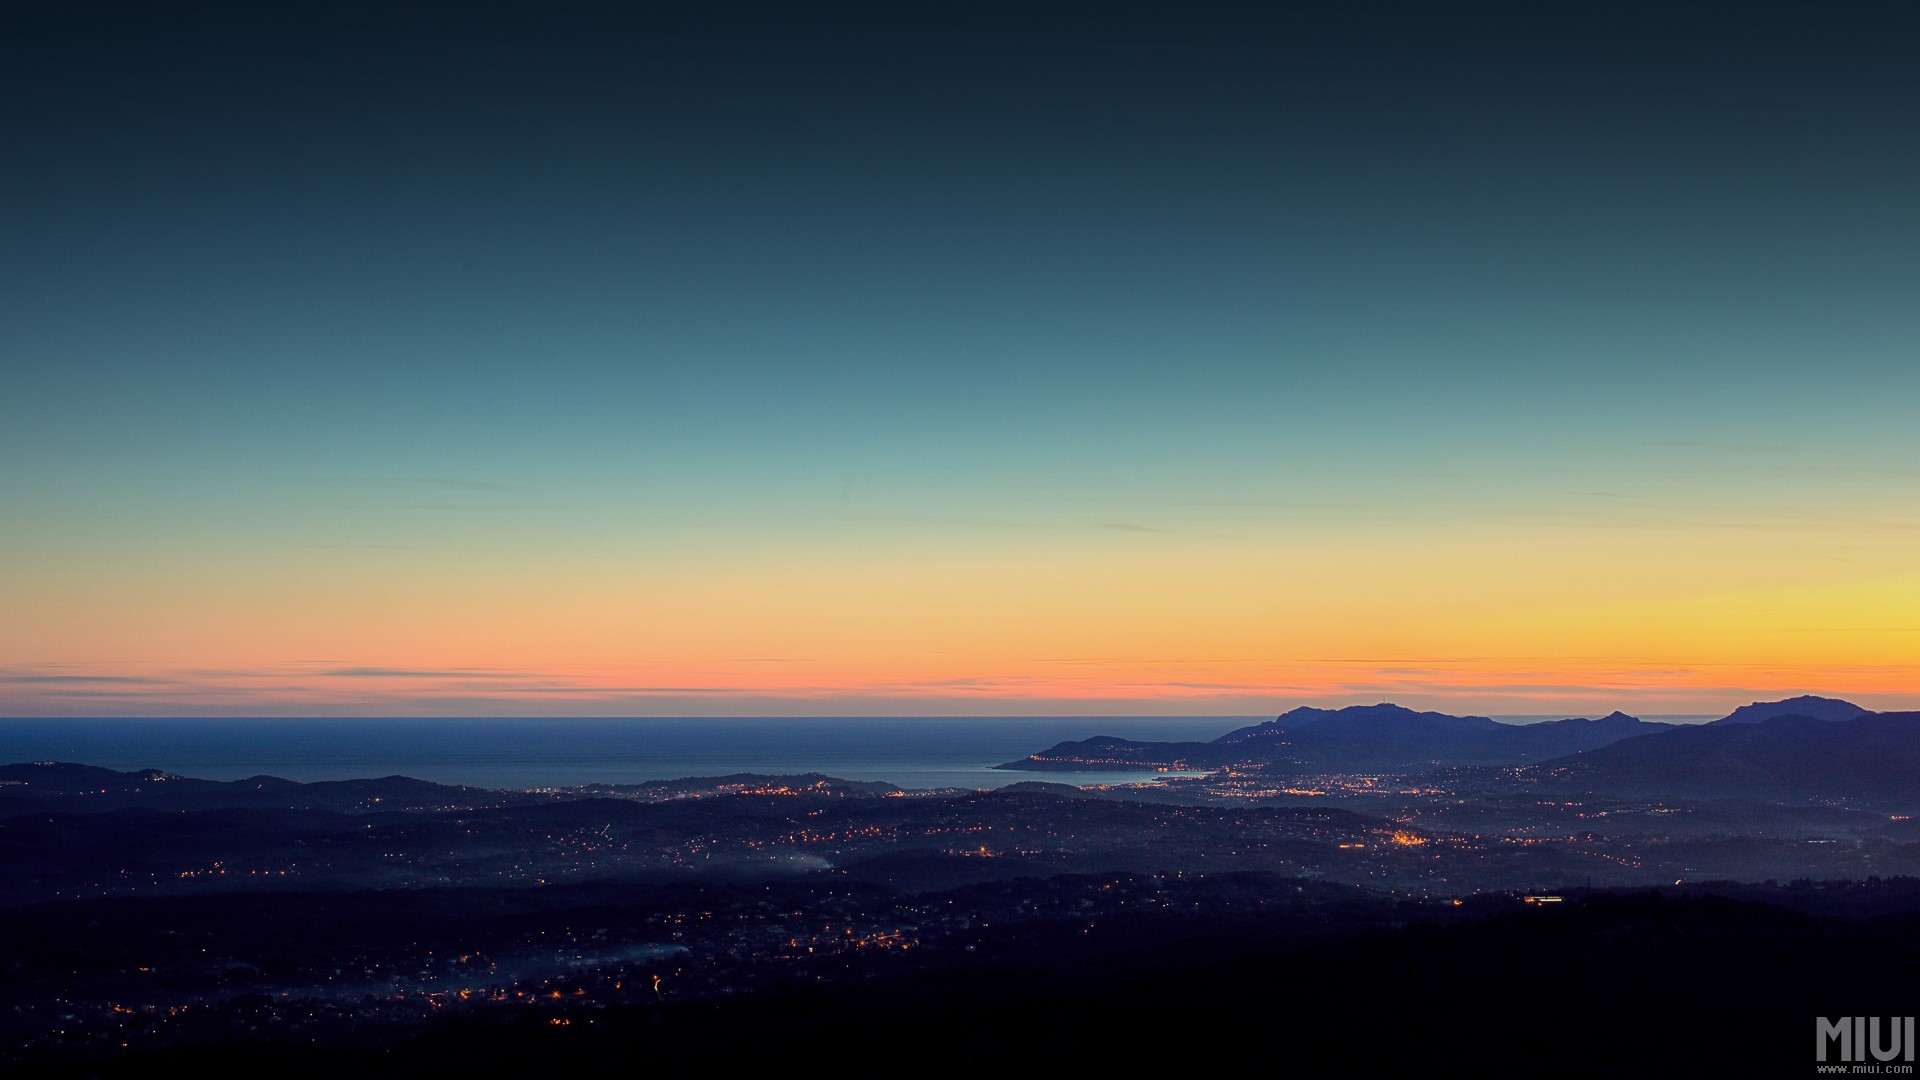
\includegraphics[width=1\textwidth]{figure/demo.jpg}		
	\end{minipage}	
	\begin{minipage}[c]{0.5\textwidth}		
		\centering		
		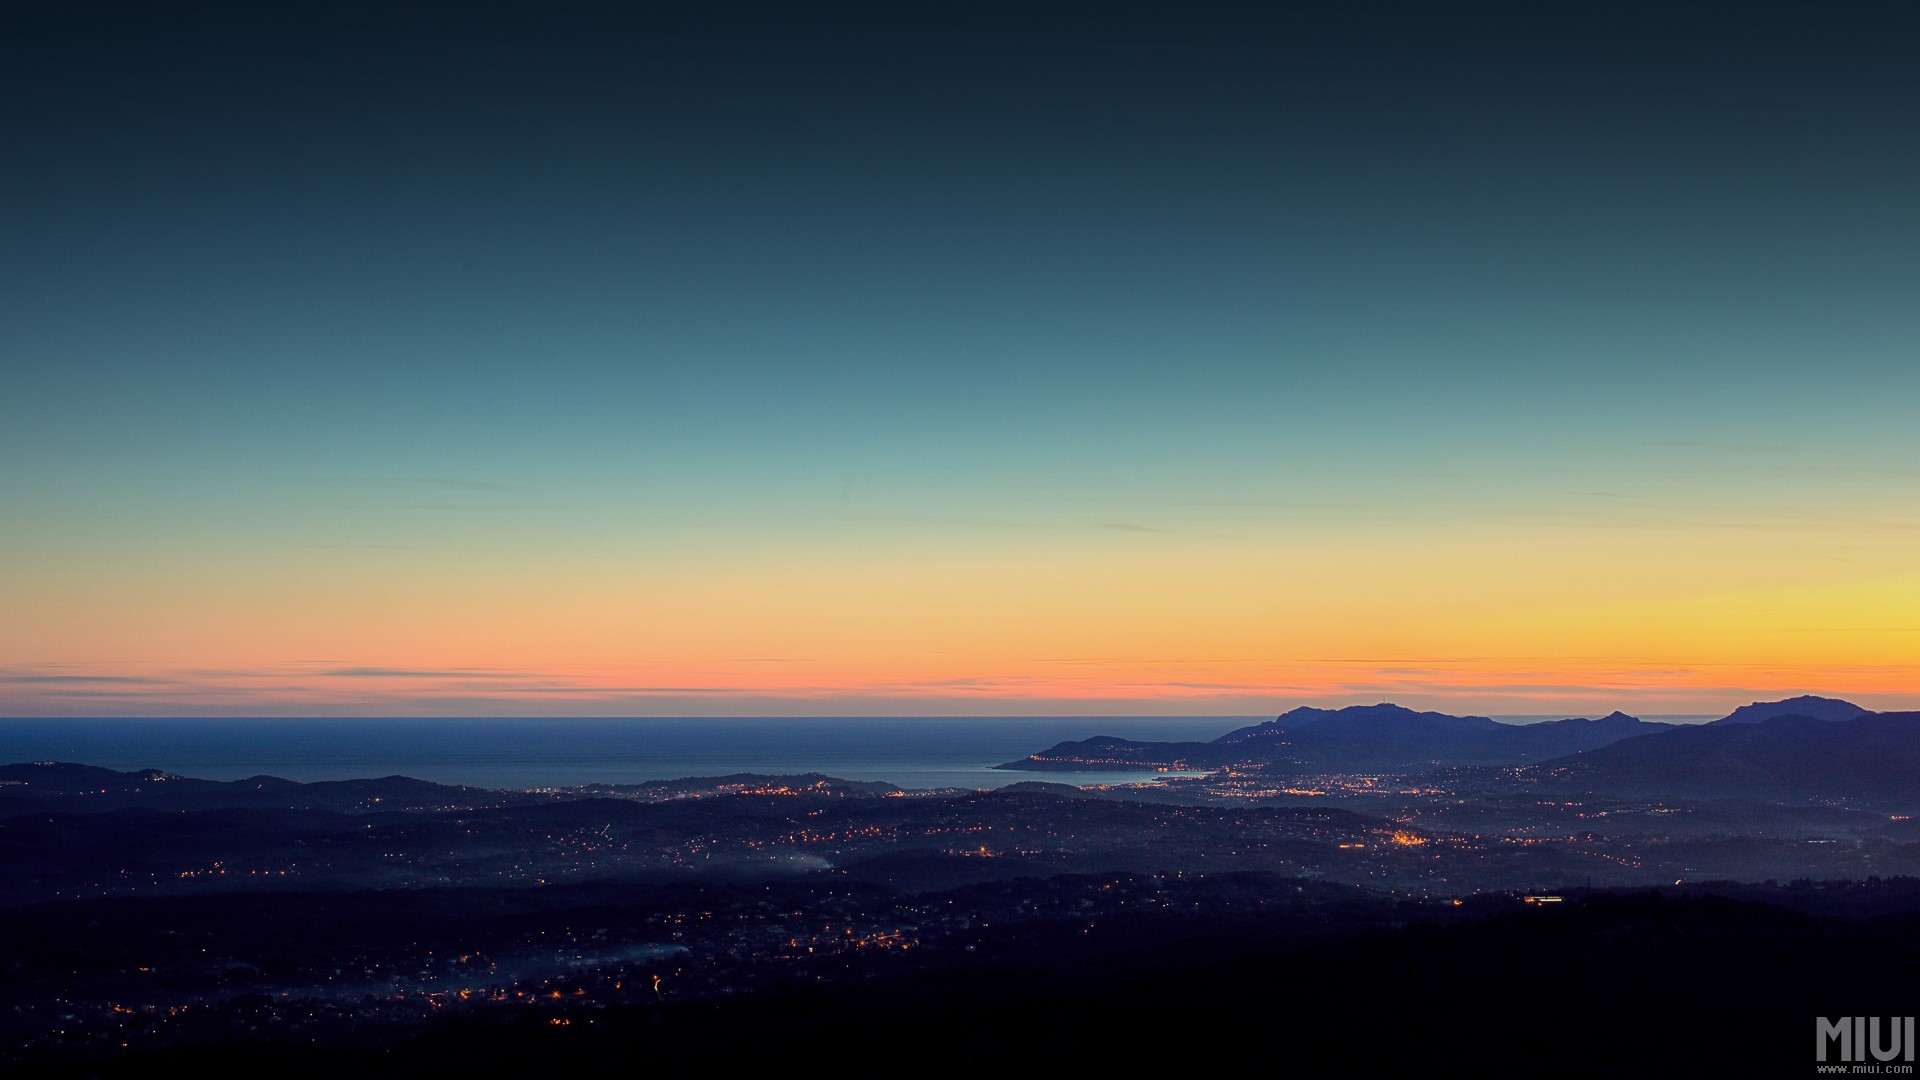
\includegraphics[width=1\textwidth]{figure/demo.jpg}		
	\end{minipage}	
	\caption{水平插入两张图片}	
\end{figure}

竖直插入两张图片

\begin{figure}	
    \centering	
	\begin{minipage}{0.5\textwidth}		
		\centering		
		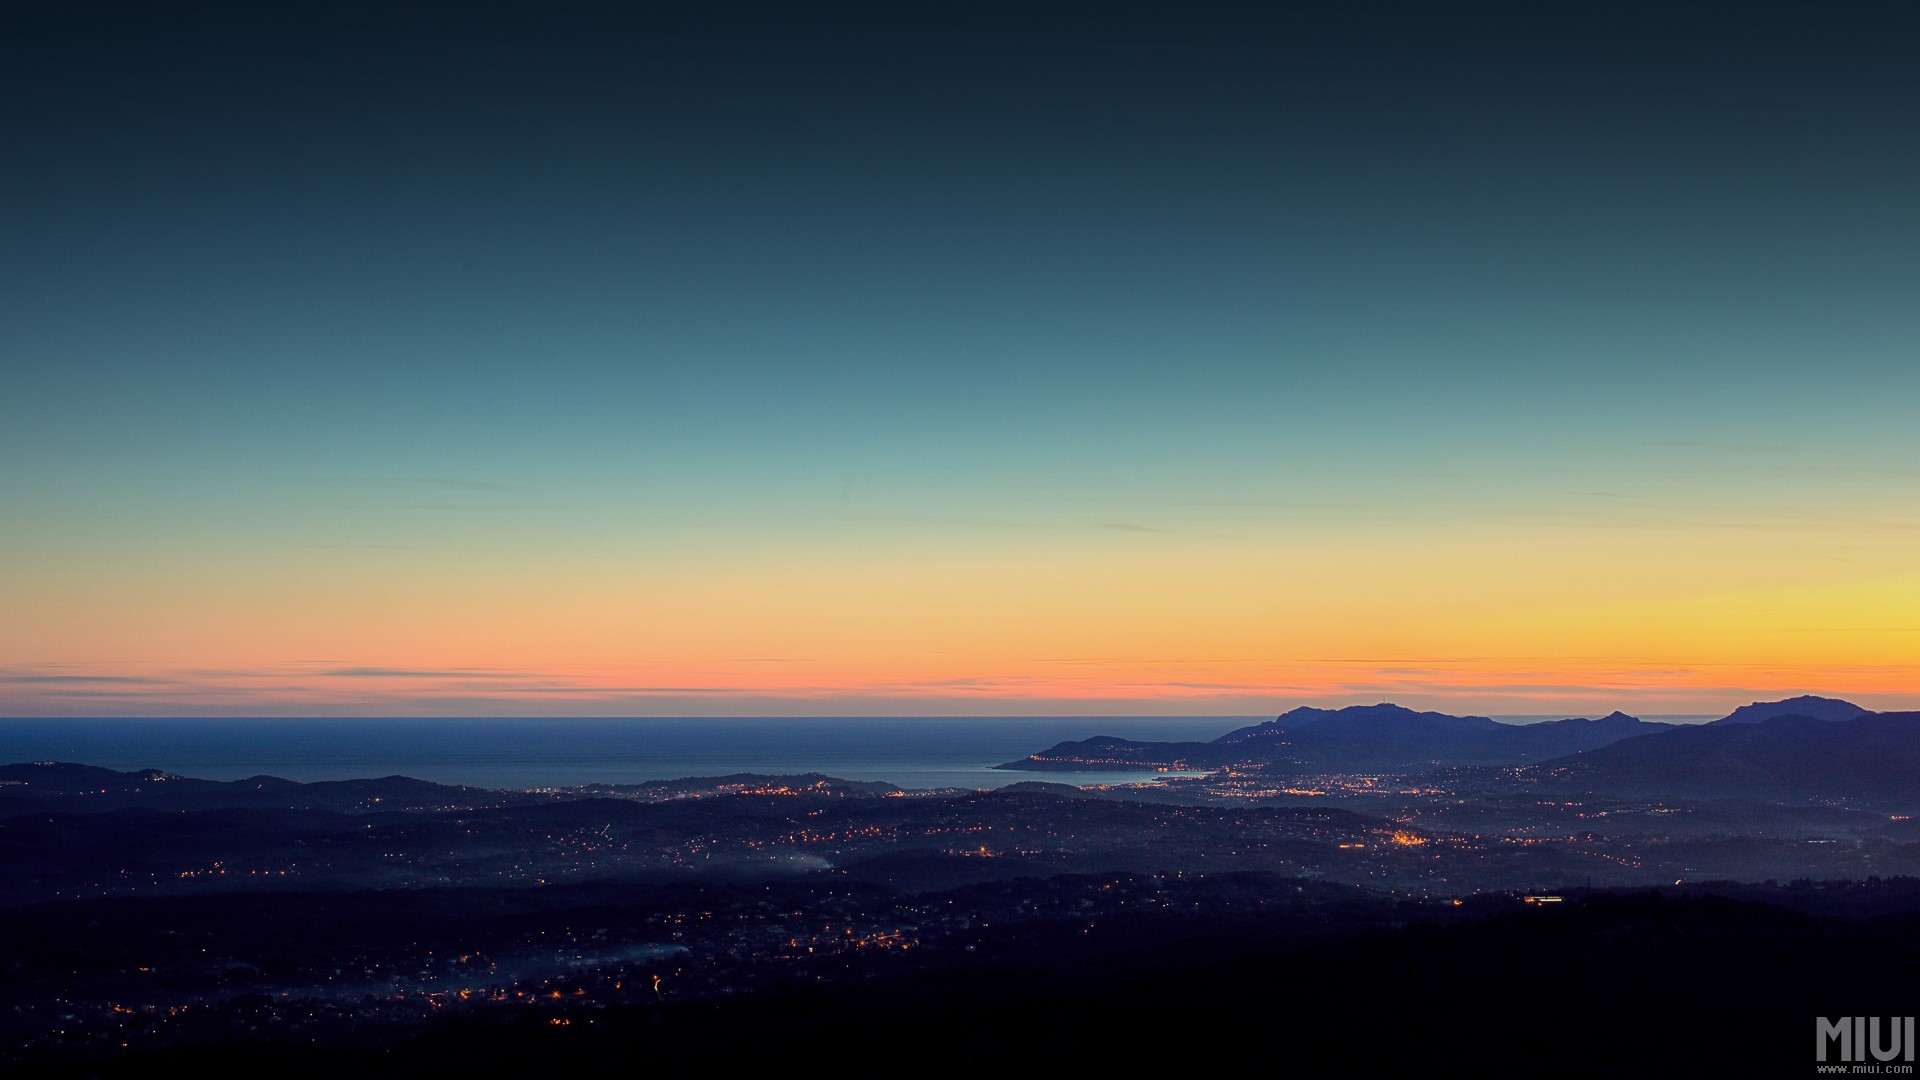
\includegraphics[height=4.5cm]{figure/demo.jpg}		
	\end{minipage}
	
	\begin{minipage}{0.5\textwidth}		
		\centering		
		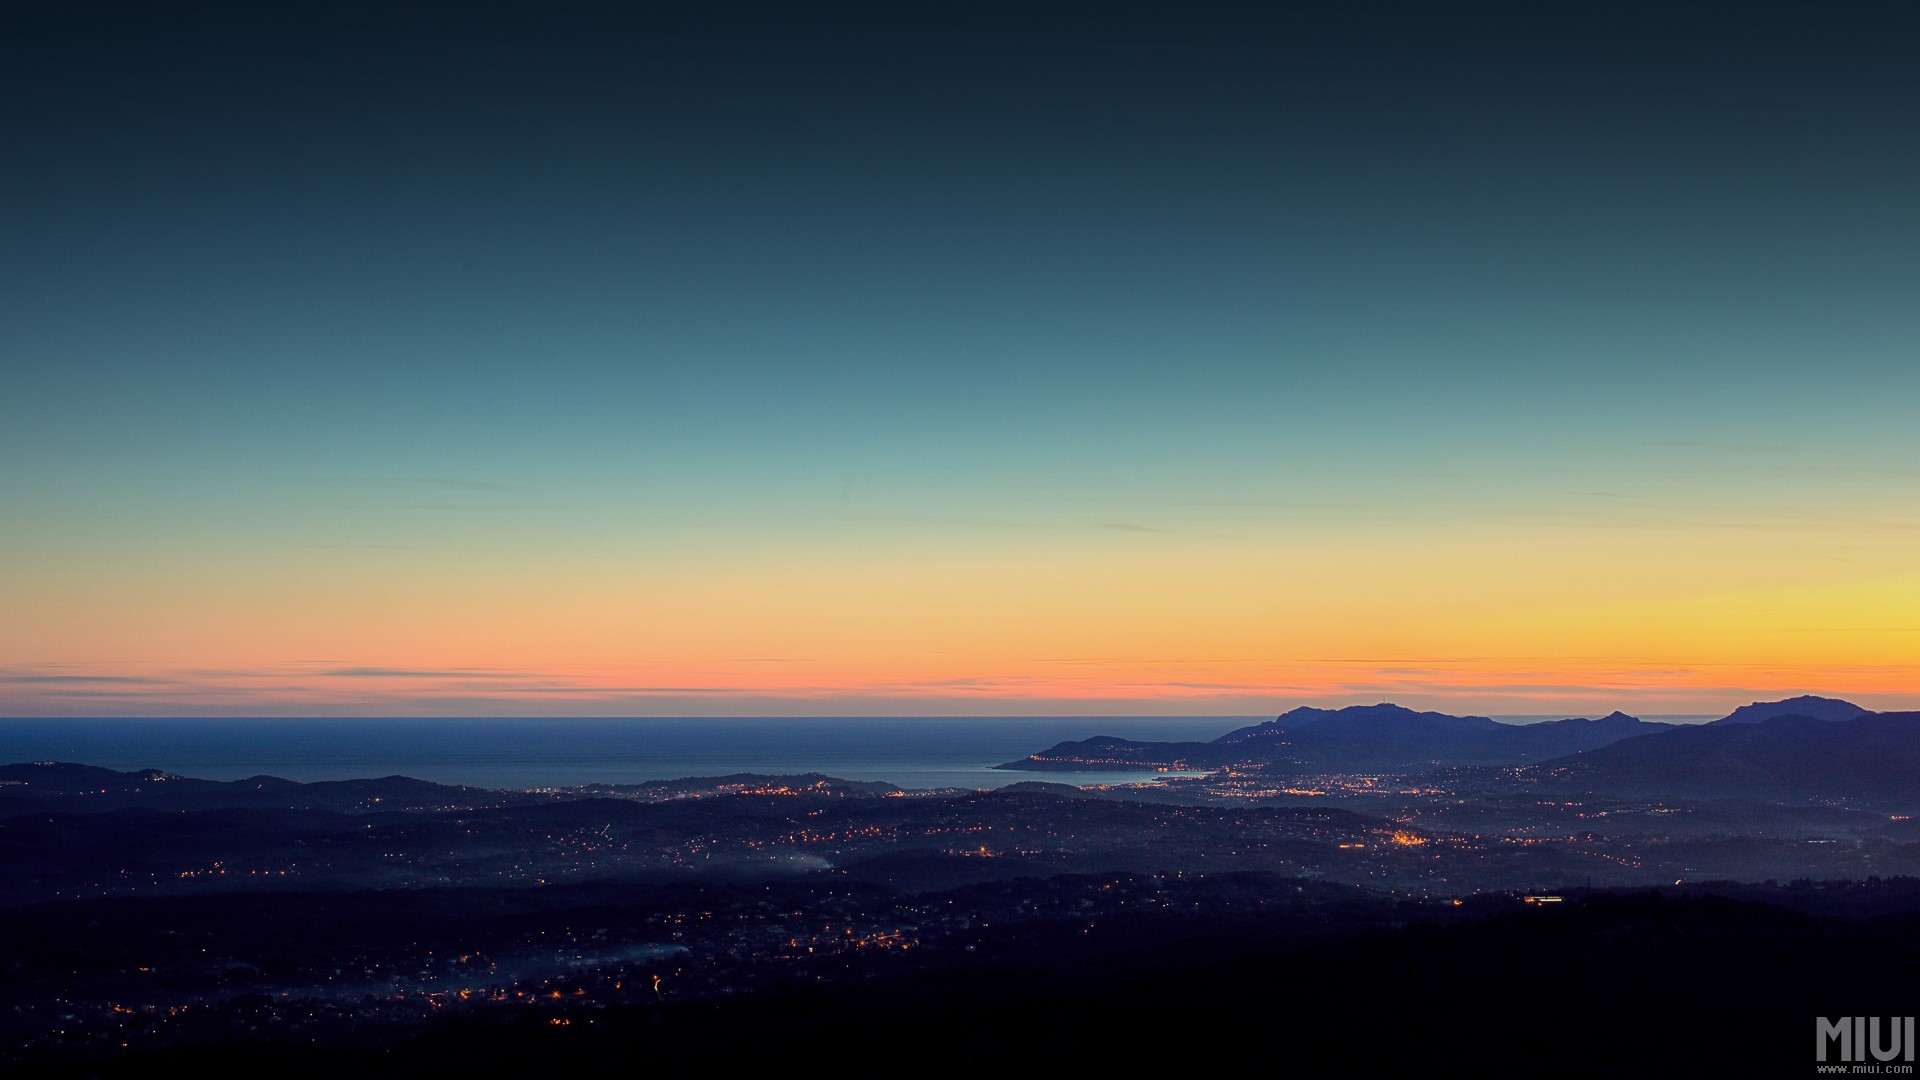
\includegraphics[height=4.5cm]{figure/demo.jpg}		
	\end{minipage}	
	\caption{竖直插入两张图片}	
\end{figure}


\newpage






\section{插表}
\subsection{三线表的排版}
\renewcommand{\tablename}{表}
\begin{table}[htbp]
	\centering
	\caption{demo}\label{table1}
	\begin{tabular}{ccc}    
		\toprule            
		1 & 2 & 3 \\        
		\midrule            
     	1 & 2 & 3 \\
        4 & 5 & 6 \\
		\bottomrule         
	\end{tabular}
\end{table}

According to the Table \ref{table1}, we can see that...


\subsection{合并单元格的方法}
\subsubsection{水平方向}

\begin{table}[htbp]
\centering
\begin{tabular}{|c|c|c|}
	\hline
	1 & 2 & 3 \\
	\hline
	\multicolumn{2}{|r}{x} & \multicolumn{1}{|l|}{y} \\
	\hline
	4 & \multicolumn{2}{c|}{z} \\
	\hline
\end{tabular}
\end{table}

\subsubsection{垂直方向(multirow)}



\begin{table}[htbp]
\centering
\begin{tabular}{cc}
	\hline
	\multirow{3}{*}{text} & item1  \\
	& item2  \\
	& item3  \\
	\hline
\end{tabular}
\end{table}



\subsection{带斜线的表格}
\begin{table}[htbp]
	\caption{带斜线的表格}
	\centering
	\begin{tabular}{|c|cc|}
		\hline
		\diagbox{1}{2} & A & B \\   %斜线命令语句
		\hline
		1 & 2 & 3 \\
		4 & 5 & 6 \\
		7 & 8 & 9 \\
		\hline
	\end{tabular}
\end{table}

\section{浮动体}

内容丰富的文章或者书籍往往包含许多图片和表格等内容。这些内容的尺寸往往太大,导致分页困难。\LaTeX 为此引入了浮动体的机制,令大块的内容可以脱离上下文,放置在合适的位置。

% h -当前位置
% t -顶部
% b -底部
% p -单独一页
% ! -忽略限制

% 常用的顺序优先级 htbp



\subsection{大标题+子标题}

%\begin{figure}[htbp]
\begin{figure}[tbp]
	\centering
	\subfloat[fig1]{
		\label{sub-figure7a}
		\begin{minipage}{0.5\textwidth}
			\centering
			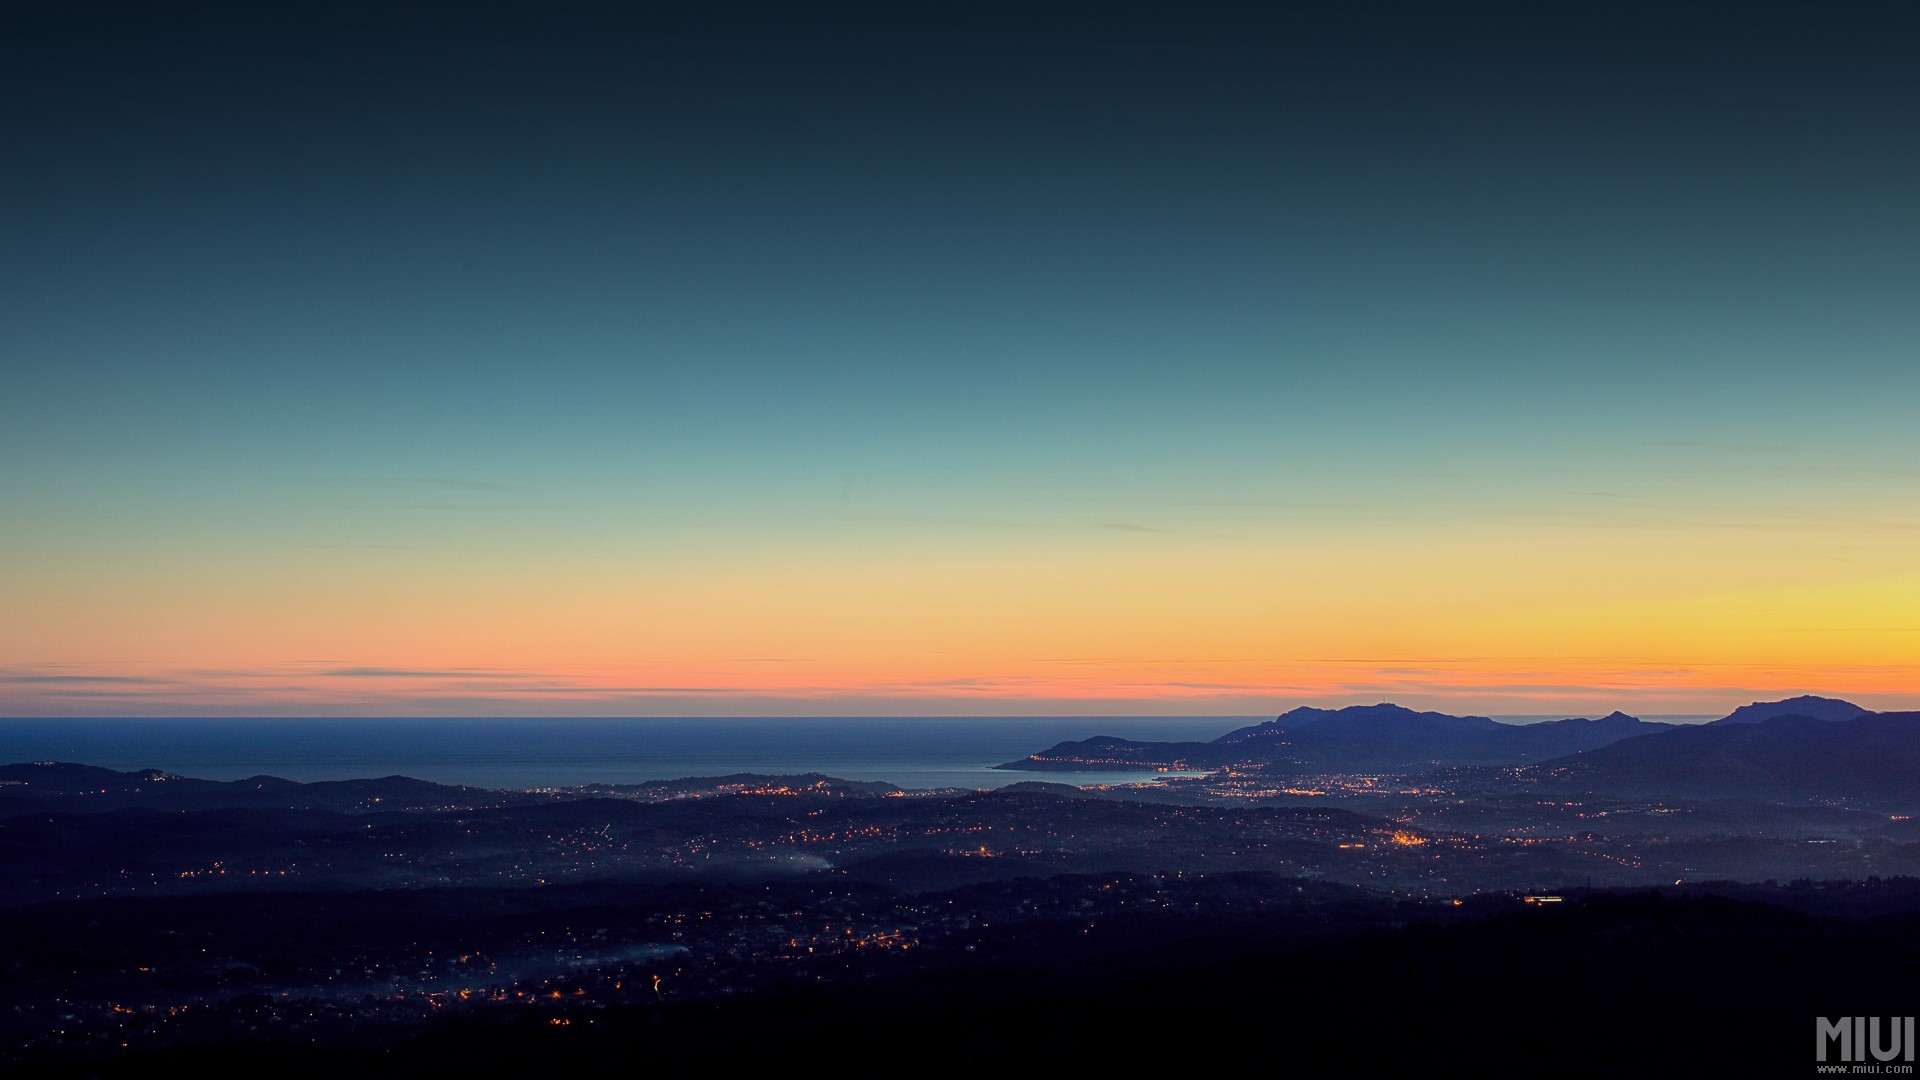
\includegraphics[width=0.5\linewidth]{figure/demo.jpg}
		\end{minipage}	
	}
	\qquad
	\subfloat[fig2]{
		\label{sub-figure7b}
		\begin{minipage}{0.5\textwidth}
			\centering
			
\includegraphics[width=0.5\linewidth]{figure/demo1.jpg}
		\end{minipage}	
	}
	\caption{子标题举例}
	\label{figure7}
\end{figure}

this is the figure \ref{figure7} and it contains two pictures which are figure \ref{sub-figure7a} adn \ref{sub-figure7b}.

\subsection{单独的标题}

\begin{figure}[htpb]
	\centering
	\begin{minipage}{0.5\textwidth}
		\centering
		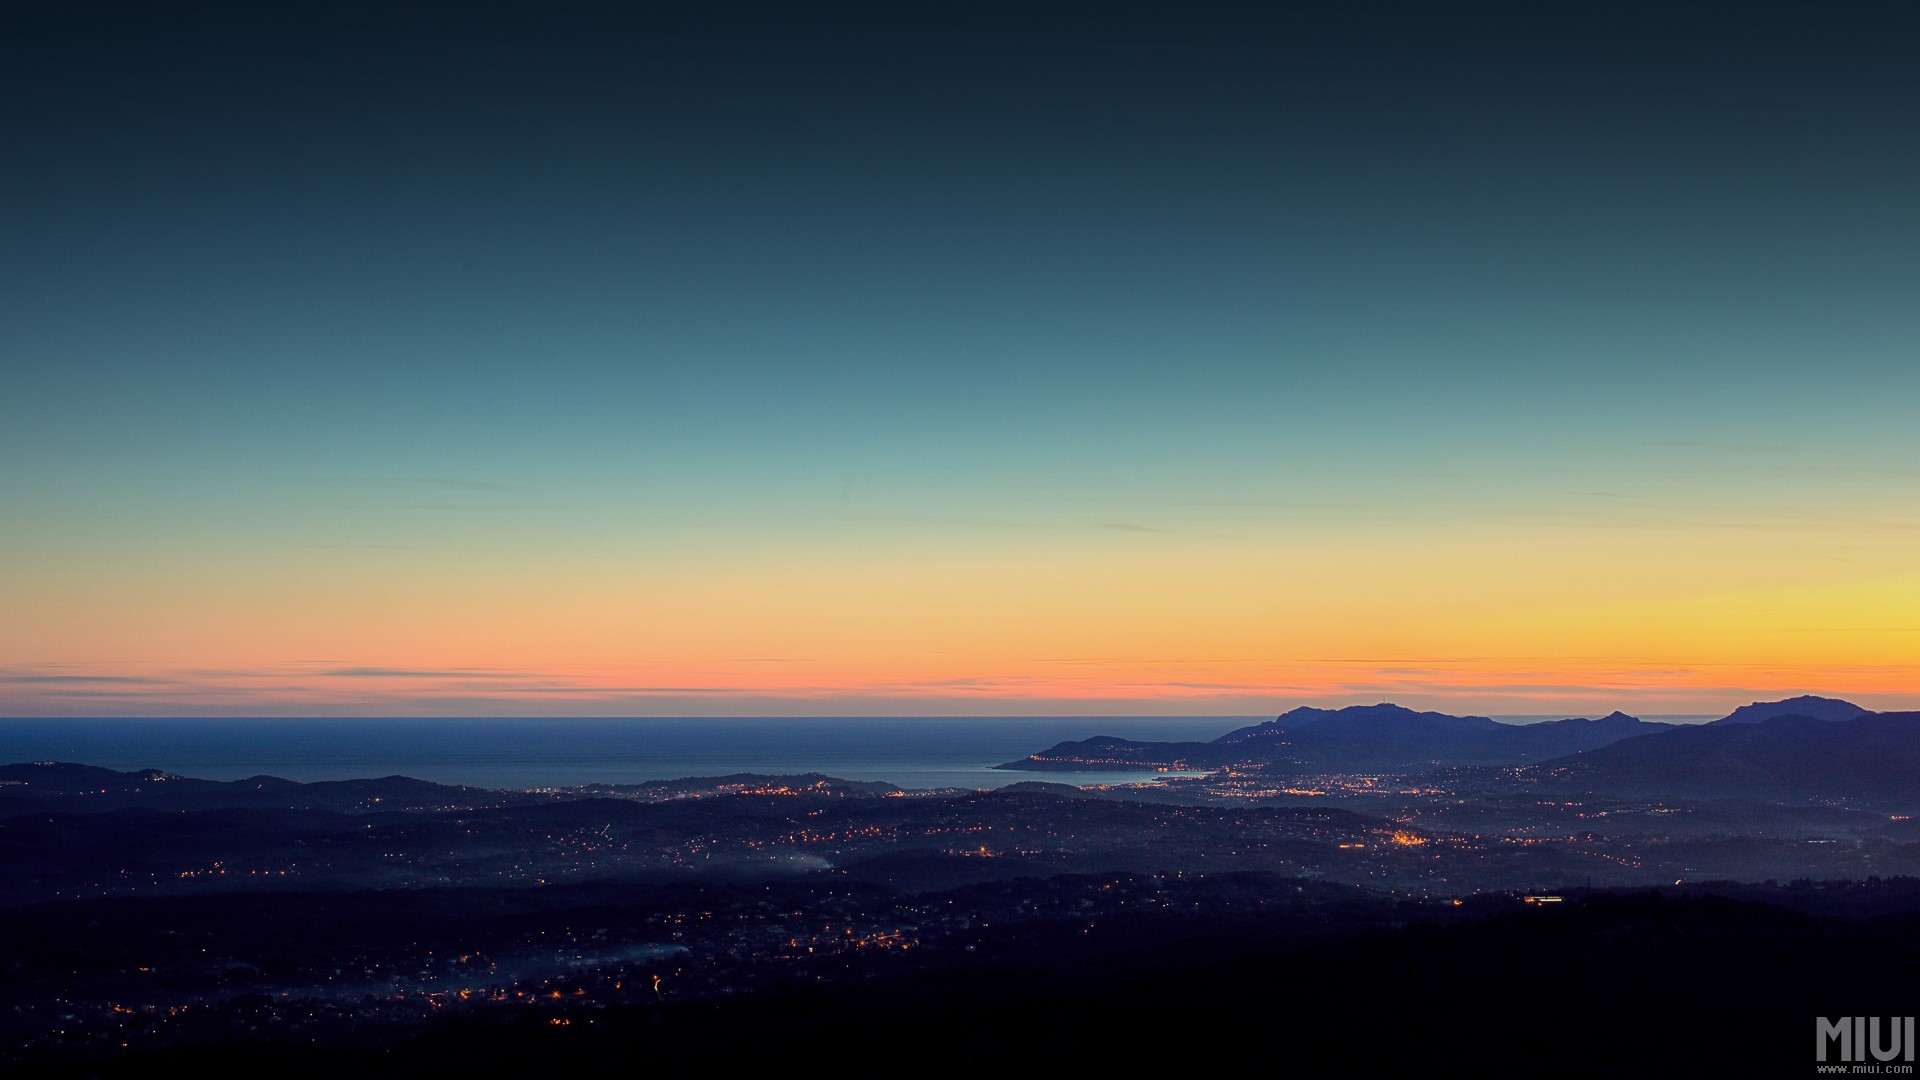
\includegraphics[width=4cm]{figure/demo.jpg}
		\caption{fig3}
		\label{figure8}
	\end{minipage}
    \qquad
    \begin{minipage}{0.5\textwidth}
        \centering
        
\includegraphics[width=4cm]{figure/demo1.jpg}
        \caption{fig4}
        \label{figure9}
    \end{minipage}
\end{figure}
	
\ref{figure8} and \ref{figure9}	

\section{将excel表格转换为latex代码}
使用excel插件:Excel2LaTeX

插件下载网址:https://ctan.org/tex-archive/support/excel2latex/

\begin{figure}	
	\centering	
	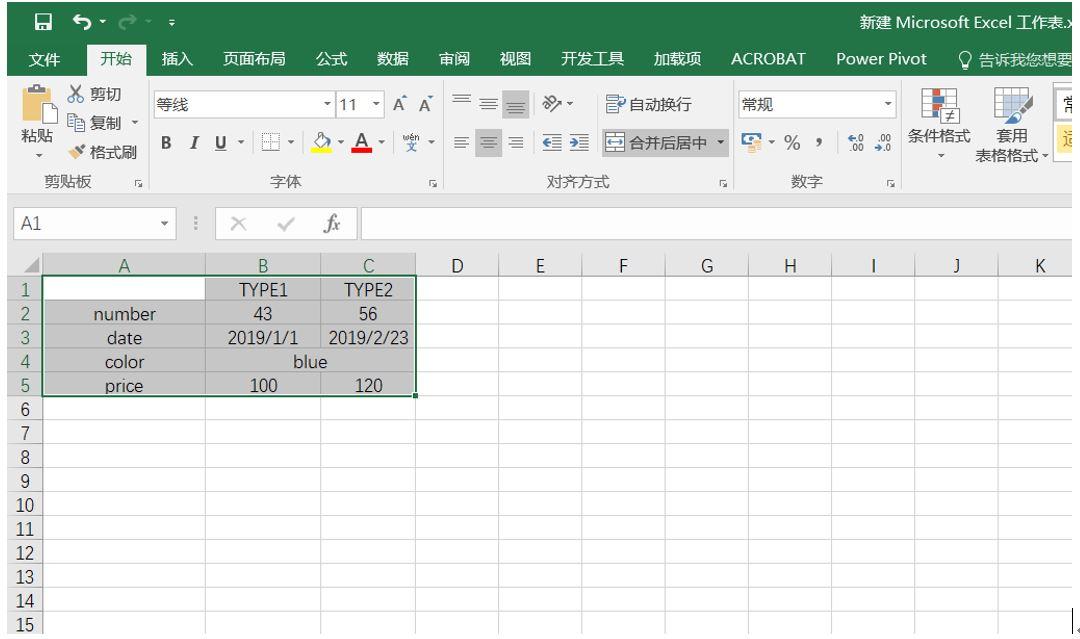
\includegraphics[width=\linewidth]{figure/excel1.jpg}	
\end{figure}

\begin{figure}	
	\centering	
	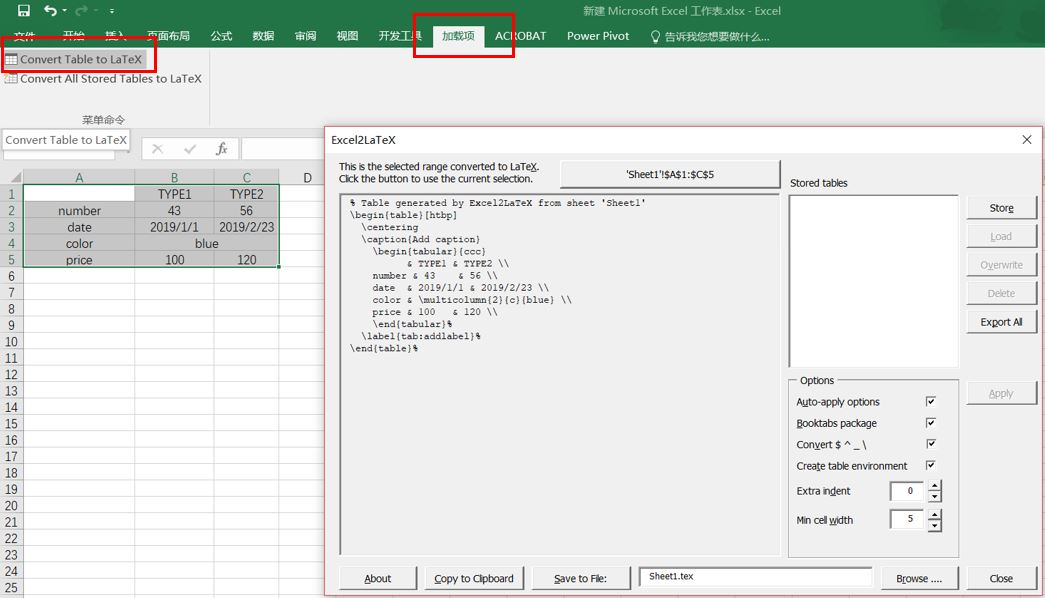
\includegraphics[width=\linewidth]{figure/excel2.jpg}	
\end{figure}

\begin{figure}	
	\centering	
	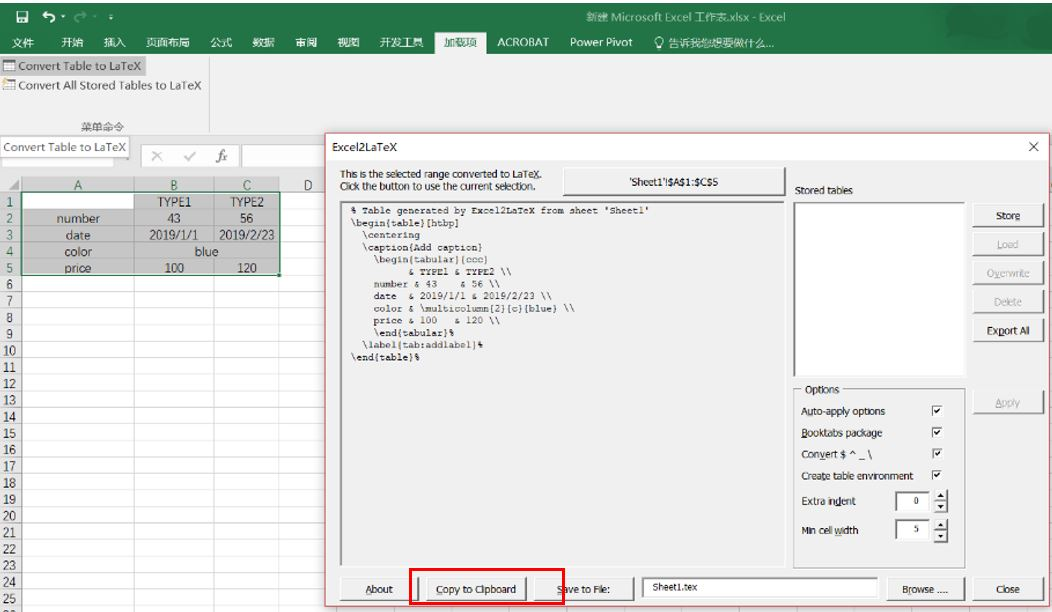
\includegraphics[width=\linewidth]{figure/excel3.jpg}	
\end{figure}

\end{document}


